\section{Classification}

\subsection{Introduction}

The idea is to learn a classifier, which is usually a function mapping from an input data point to one of a set of discrete outputs, i.e., the classes.

\begin{itemize}
    \item Does the algorithm require all training data to be present before the start of learning? If yes, then it is categorised as \textbf{batch learning} algorithm.
    \item If however, it can continue to learn a new data arrives, it is an \textbf{online learning} algorithm.
    \item If the model has a fixed number of parameters it is categorised as \textbf{parametric}.
    \item Otherwise if the number of parameters grows as part of training it is categorised as \textbf{non-parametric}.
\end{itemize}

\subsection{Evaluating Classification}

Classification accuracy on a sample of labelled pairs \((x, c(x))\) given a learned classification model that predicts, for each instance \(x\), a class value \(\hat{c}(x)\):

\[\mathrm{acc} = \frac{1}{|\mathrm{Test}|} \sum_{x \in \mathrm{Test}} I[\hat{c}(x) = c(x)]\]

where Test is a test set and \(I[]\) is the indicator function which is 1 if and only if its argument evaluates to true, and 0 otherwise. Classification error is 1-acc. \\

For the two-class prediction case:

\begin{itemize}
    \item Two kinds of error (incorrect classification):
    \begin{itemize}
        \item False Positive and False Negative may have different costs.
    \end{itemize}
    \item Two kinds of correct classification:
    \begin{itemize}
        \item True Positive and True Negative may have different ``benefits''.
    \end{itemize}
    \item Note: total number of test set examples \(N = TP + FN + FP + TN\)
\end{itemize}

\subsection{Perceptron}

Output \(o\) is thresholded sum of products of inputs and their weights:

\[o(x_1, \dots, x_n) = \begin{cases}
    +1 & \text{ if } w_0 + w_1x_1 + \cdots + w_nx_n > 0 \\
    -1 & \text{ otherwise}.
\end{cases}\]

Or in vector notation:

\[o(\vecx) = \begin{cases}
    1 & \text{ if } \vec{w} \cdot \vecx > 0 \\
    -1 & \text{ otherwise.}
\end{cases}\]

\textbf{Key idea:} Learning is ``finding a good set of weights''. Perceptron learning is simply an iterative weight-update scheme:

\[w_i \leftarrow w_i + \Delta w_i\]

where the weight update \(\Delta w_i\) depends only on misclassified examples and is modulated by a ``smoothing'' parameter \(\eta\) typically referred to as the ``learning rate''.

\begin{itemize}
    \item We combine the misclassified positive and negative cases with a single update rule:
    \[\vec{w}' + \vec{w} + \eta y_i \vecx_i\]
    \item Here \(y_i\) acts to change the sign of the update, corresponding to whether a positive or negative example was misclassified.
\end{itemize}

The algorithm just iterates over the training examples applying the weight update rule until all the examples are correctly classified.

\begin{center}
    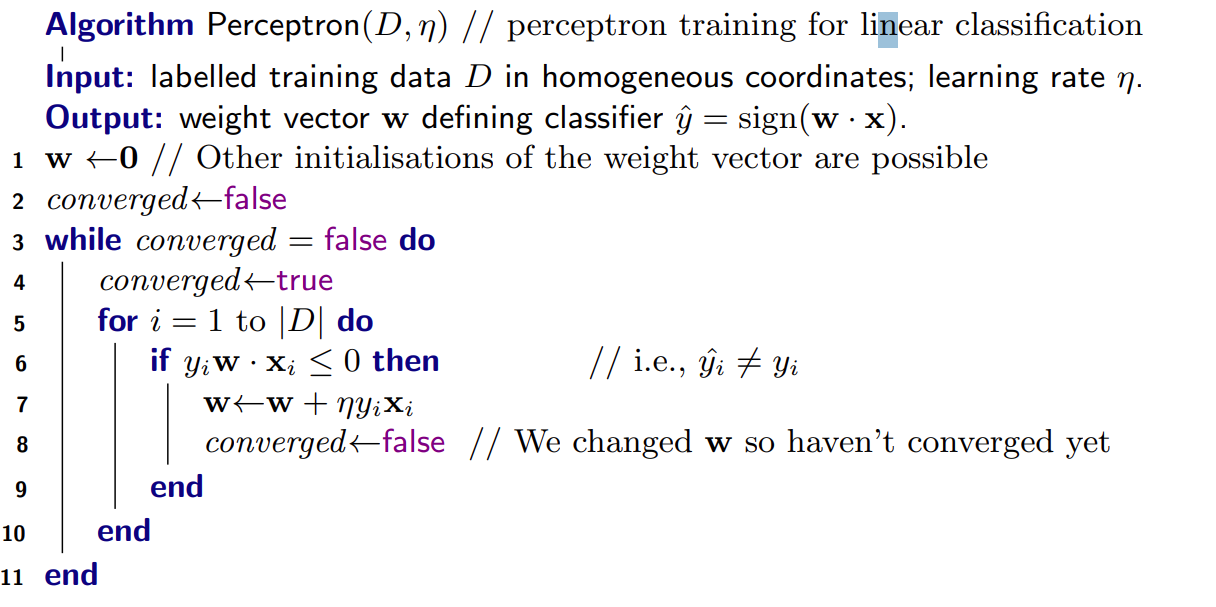
\includegraphics[scale=0.6]{./assets/perceptron.png}
\end{center}

Perceptron training will converge (under some mild assumptions) for linearly separable classification problems. A labelled data set is linearly separable if there is a linear decision boundary that separates the classes.

\subsection{Logistic Regression}

In the case of a two-class classification problem, if we model the probability \(P(Y = 1)\) of an instance \(\vecx\) being a positive example like this:
\[P(Y = 1 \mid \vecx) = \frac{1}{1 + e^{-\vec{w}^\top \vecx}}\]
then this probability vs. the alternative \((1 - P(Y = 1))\) can be written like this:
\[\ln \frac{P(Y = 1 \mid \vecx)}{1 - P(Y = 1 \mid \vecx)} = \vec{w}^\top \vecx\]

The quantity on the LHS is called the logit and we are defining a linear model for the logit. \\

An iterative gradient ascent method can be used to maximise log likelihood. The (conditional) log likelihood is
\[\sum_{i = 1}^N y^{(i)}\log P(1 \mid \vec{x}^{(i)}) + (1 - y^{(i)}) \log (1 - P(1 \mid \vecx^{(i)})).\]
Over a set of \(N\) examples, choose \(\vec{w}\) to maximise this expression, noting that \(y^{(i)}\) is always either 0 or 1.

\subsection{Bayes Theorem and Maximum Likelihood}

Bayes Theorem for estimating probability of model \(m\) from data \(D\):

\[P(m \mid D) = \frac{P(D \mid m)P(m)}{P(D)}\]
where
\begin{flalign*}
    \qquad & P(m) = \text{prior probability of model} m &&\\
    \qquad & P(D) = \text{prior probability of training data } D &&\\
    \qquad & P(m \mid D) = \text{ probability of } m \text{ given } D &&\\
    \qquad & P(D \mid m) = \text{ probability of } D \text{ given } m &&
\end{flalign*}

Maximum a posteriori hypothesis \(m_{MAP}\):
\begin{align*}
    m_{MAP} &= \arg\max_{m \in \mathcal{M}} P(m \mid D) \\
    &= \arg \max_{m \in \mathcal{M}} \frac{P(D \mid m)P(m)}{P(D)} \\
    &= \arg \max_{m \in \mathcal{M}} P(D \mid m)P(m)
\end{align*}

If assume \(P(m_i) = P(m_j)\) then can further simplify, and choose the Maximum Likelihood (ML) hypothesis
\[h_{ML} = \arg \max_{m_i \in \mathcal{M}} P(D \mid m_i)\]
This assumption means we believe all models are a priori equally likely. \\

\textbf{Bayes optimal classification:}
\[\arg \max_{y_i \in \mathcal{Y}} \sum_{m_i \in \mathcal{M}} P(y_j \mid m_i) P(m_i \mid D)\]

\textbf{Problem:} Bayes optimal classification is typically intractable and is therefore not used in practice!